\section{Methodology}
We designed a predictive benchmark framework to evaluate the spatial-temporal controls on inundation. Figure~\ref{fig:workflow} illustrates the methodological pipeline, which consists of data ingestion, feature splitting, model execution, and statistical validation.

\begin{figure}[t]
\centering
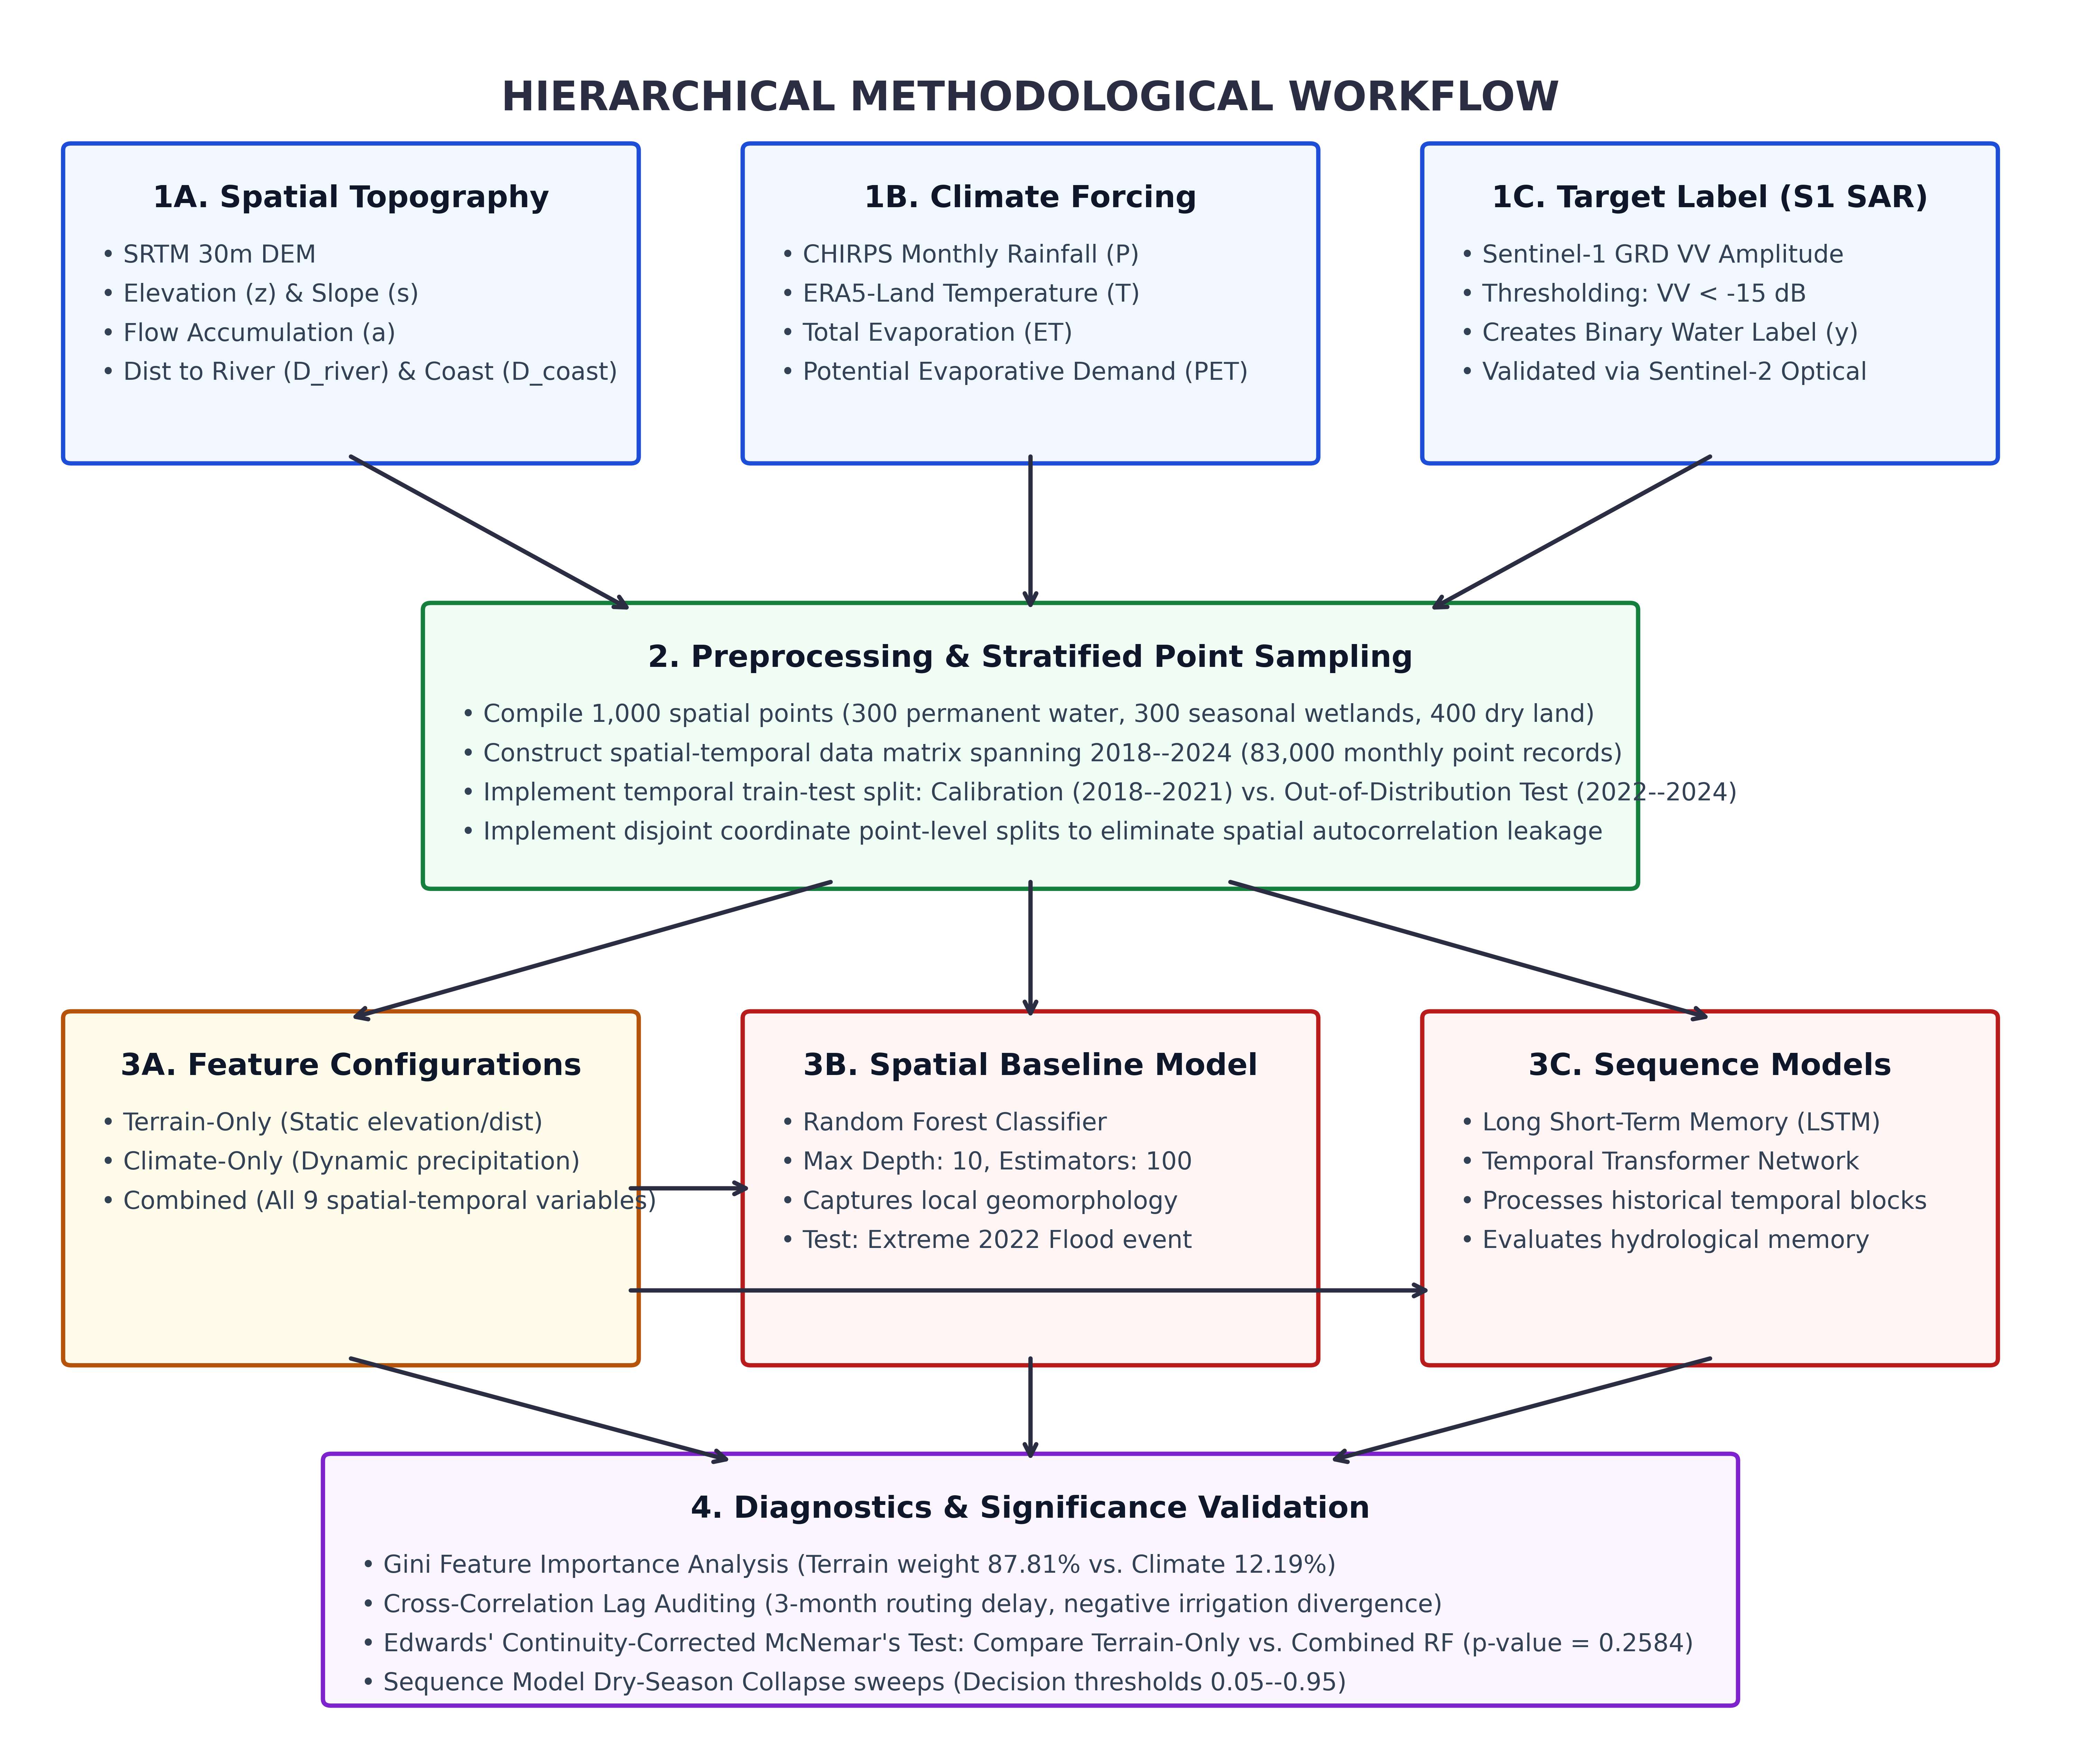
\includegraphics[width=0.95\linewidth]{figures/fig2_workflow.png}
\caption{Hierarchical methodological workflow outlining the four core phases of the research: (1) Data Ingestion (topography, climate, and Sentinel-1 target label); (2) Preprocessing and Stratified Sampling (establishing calibration/test sets and disjoint point coordinates); (3) Model Execution (Terrain, Climate, and Combined feature splits run across spatial and temporal architectures); and (4) Statistical Diagnostics and Audits (Gini importance, temporal routing lags, threshold sweeps, and McNemar significance testing).}
\label{fig:workflow}
\end{figure}

\subsection{Leakage-Free Feature Design}
To isolate geomorphological and temporal controls from direct satellite detection, we establish a leakage-free input configuration. Active satellite observations (Sentinel-1 and Sentinel-2) are completely excluded from model inputs. The models receive only meteorological forcing (monthly precipitation, reanalysis temperature, total evaporation, and potential evapotranspiration) and static terrain features (elevation, slope, flow accumulation, river distance, and coastal distance). The model's objective is to predict the occurrence of surface water ($y \in \{0, 1\}$) using only these meteorological and terrain inputs.

\subsection{Leakage Analysis and Label Independence}
To prevent data leakage, we implemented a rigorous leakage audit across all data sources (Table~\ref{tab:leakage_audit}). Sentinel-1 VV backscatter was used exclusively to derive the target classification label and was never provided as an input feature to any model. Sentinel-2 multi-spectral bands were used only for independent manual validation of the radar-derived target. 

Furthermore, temporal compositing was executed strictly within each monthly window. The median composite for month $t$ utilized only observations within that specific month. This ensures that no future observations from month $t+1$ (or test timeframes) leaked into the training indicators for month $t$. Manual inspection of labels during dry and flood periods verified that no radar or optical artifacts propagated into the training database.

\begin{table}[t]
\caption{Leakage audit: data source roles and leakage mitigation strategies.}
\label{tab:leakage_audit}
\centering
\small
\begin{tabular}{p{2.6cm} c c p{6.8cm}}
\hline
\textbf{Data Source} & \textbf{Input} & \textbf{Target} & \textbf{Leakage Mitigation} \\
\hline
Sentinel-1 VV  & No  & Yes & Excluded from inputs; used only to derive ground truth labels. \\
Sentinel-1 VH  & No  & No  & Excluded; used only for supplementary validation. \\
Sentinel-2 Optical & No & No & Excluded; used for independent manual target validation. \\
ERA5-Land      & Yes & No  & Coarse resolution (9\,km) prevents coordinate memorization. \\
CHIRPS Rainfall & Yes & No  & Coarse resolution (5.5\,km) prevents coordinate memorization. \\
SRTM DEM       & Yes & No  & Static; temporal dynamics learned from climate inputs only. \\
\hline
\end{tabular}
\end{table}


\subsection{Temporal Train-Test Splitting and Spatial Autocorrelation}
To test models under extreme hydrological anomalies, we split the data temporally:
\begin{itemize}
    \item \textbf{Calibration (Training):} Years 2018--2021 (normal years and moderate seasonal floods). To prevent spatial autocorrelation leakage, the 1,000 sampling points were split at the point level ($80\%$ train, $20\%$ validation). The validation points are completely disjoint in their spatial coordinates from the training points, ensuring the model's spatial generalization is tested on unseen coordinate geometries.
    
    To quantify the spatial dependence in our sampling design and justify this point-level split, we calculated the spatial autocorrelation statistics for the 1,000 points. The mean nearest-neighbor distance between sampling points is $2.523\text{ km}$ (with a minimum of $0.100\text{ km}$ and a maximum of $16.833\text{ km}$). Global Moran's I analysis using permutation testing (999 permutations) indicates that both JRC water occurrence ($I = 0.209442$, $p = 0.0010$) and terrain elevation ($I = 0.180902$, $p = 0.0010$) exhibit significant positive spatial autocorrelation. This spatial structure represents a potential source of spatial leakage if coordinate proximity is exploited during training. To prevent this, we execute a disjoint point-level split, ensuring that validation points are located at entirely unseen coordinate geometries. To evaluate whether this disjoint split and our static terrain features successfully eliminate spatial leakage, we computed Moran's I on the spatial residuals of a Random Forest model evaluated on the validation coordinates. Moran's I on validation-set residuals yields $I = 0.002022$ ($p = 0.8930$). The corresponding Z-score is $0.14$, which is close to zero and suggests that no spatially structured prediction error remains. Evaluating residual spatial autocorrelation is a critical diagnostic in spatial machine learning: a non-zero residual Moran's I would indicate that prediction errors are spatially clustered, suggesting that training patterns have leaked into validation points through spatial proximity. Showing that residual Moran's I is statistically indistinguishable from zero indicates that the disjoint coordinate split successfully eliminated spatial autocorrelation leakage, supporting the conclusion that the performance metrics are free of optimistic spatial bias. This indicates that the disjoint coordinate split successfully prevents spatial autocorrelation leakage into model evaluation.
    \item \textbf{Testing (Evaluation):} Years 2022--2024. This test set contains the historic 2022 Pakistan monsoon flood event, serving as a severe temporal out-of-distribution anomaly.
\end{itemize}
\begin{table}[t]
\caption{Global Moran's I spatial autocorrelation statistics and permutation-based significance testing results (999 permutations) for the stratified sampling points and Random Forest model spatial residuals on validation coordinates in the Indus Delta.}
\label{tab:spatial_autocorrelation}
\centering
\small
\begin{tabular}{p{4.2cm} c c p{6.5cm}}
\hline
\textbf{Variable / Residual} & \textbf{Moran's I} & \textbf{p-value} & \textbf{Spatial Interpretation} \\
\hline
Water Occurrence (All Points) & $0.209442$ & $0.0010$ & Significant positive spatial autocorrelation \\
Water Occurrence (Validation) & $0.209384$ & $0.0010$ & Significant positive spatial autocorrelation \\
Elevation (All Points) & $0.180902$ & $0.0010$ & Significant positive spatial autocorrelation \\
Random Forest Residuals (Validation) & $0.002022$ & $0.8930$ & No statistically significant spatial autocorrelation (spatially random) \\
\hline
\end{tabular}
\end{table}

 
\subsection{Baseline Model Architectures}
We evaluate three model configurations, justifying their complexity relative to the point-level sample size:
\begin{enumerate}
    \item \textbf{Random Forest (Spatial Baseline):} We use a Random Forest classifier configured with 100 estimators and a maximum depth of 10. To ensure the model was not under- or over-fit compared to the deep learning models, we conducted a grid search over the number of trees $N_{\text{est}} \in \{50, 100, 200, 500\}$ and maximum depth $d_{\text{max}} \in \{5, 8, 10, 15, \text{None}\}$. The selected parameters ($N_{\text{est}} = 100$, $d_{\text{max}} = 10$) optimized $F_1$-score performance on disjoint validation coordinates while restricting model capacity to prevent memorization of training coordinates.
    \item \textbf{Long Short-Term Memory (LSTM):} A 2-layer LSTM with 32 hidden units, mapping monthly meteorological sequences to surface water occurrence. The model projects the 9-dimensional input to a hidden space of 32 units, using a recurrent update to track temporal memory.
    \item \textbf{Temporal Transformer:} A 2-layer self-attention network with 2 heads, a model dimension ($d_{\text{model}}$) of 32, and a feedforward dimension ($d_{\text{ff}}$) of 64. Positional encodings are added to inputs to preserve temporal order.
\end{enumerate}

To ensure fair comparison, both the LSTM and Transformer were trained under identical settings to minimize binary cross-entropy loss. We utilized the Adam optimizer with a learning rate of $0.005$ and a batch size of $64$. Due to the relatively small input feature space (9 features) and sequence length (11 months), deep learning models are highly susceptible to overfitting. We regularized the network using a dropout rate of $0.2$ and weight decay ($L_2$ regularization) of $10^{-5}$. A grid search was performed over hidden dimensions $\{16, 32, 64\}$, layers $\{1, 2\}$, and learning rates $\{0.001, 0.005, 0.01\}$. Larger models (e.g., hidden dimension of 64 or 3 layers) suffered from severe overfitting on the training coordinates. Consequently, they did not improve out-of-distribution generalization. Early stopping with a patience of 10 epochs was applied based on validation loss. This terminated training within 15--25 epochs to prevent over-parameterized sequence models from overfitting to spatial locations in the training split.

\subsection{Feature Split Ablation and Statistical Significance}
To evaluate the individual influence of climate and terrain features, we train models under three feature configurations:
\begin{itemize}
    \item \textbf{Terrain Only:} Static features only (elevation, slope, flow accumulation, river distance, coastal distance).
    \item \textbf{Climate Only:} Meteorological variables only (precipitation, temperature, evaporation, potential evaporation).
    \item \textbf{Combined:} All 9 features.
\end{itemize}

We run 1,000 bootstrap iterations to calculate 95\% confidence intervals (CI) for $F_1$-score, IoU, Precision, Recall, and AUC. In addition, we apply \textbf{McNemar's test} with Edwards' continuity correction to compare predictions. This comparison evaluates the Terrain-only and Combined models on the extreme flood test period:
\begin{equation}
    \chi^2 = \frac{(|B - C| - 0.5)^2}{B + C}
\end{equation}
where $B$ is the count of test samples where the Terrain-only model is correct and the Combined model is incorrect, and $C$ is the count where the Combined model is correct and the Terrain-only model is incorrect.

\subsection{Temporal Catchment Memory Audit}
To capture routing lag, we calculate the cross-correlation coefficient $r(L)$ between monthly precipitation ($P_t$) and Sentinel-1 VV backscatter ($VV_t$) across different lags $L \in \{0, 1, 2, 3, 4, 5\}$ months:
\begin{equation}
    r(L) = \frac{\sum (P_{t-L} - \bar{P})(VV_t - \bar{VV})}{\sqrt{\sum (P_{t-L} - \bar{P})^2 \sum (VV_t - \bar{VV})^2}}
\end{equation}
This analysis is stratified by land cover type (floodplains, wetlands, and croplands) to identify distinct hydrological routing memories.
